\chapter{Experiments}
\label{chap:experiments}

All past chapters refer to the theory and name some theoretical implementation-details, all to verify the developed procedure.
However, this chapter presents some results to validate, that the spread of found paths really improves.

\section{The testing-machine and simulation-setup}

    Firstly, the used machine runs an AMD Ryzen 7 3700X 8-Core Processor and has \si{\num{32} \giga\byte} of RAM built in, although only a few \si{\giga\byte} are needed (highly dependent on the map and number of threads).
    The operation-system is Arch Linux [x86\_64] with the kernel 5.7.9-arch1-1 installed.
    The used code for this thesis can be found in \cite{github:dominicparga/osmgraphing} and is implemented in Rust.
    Python is used for the visualization.
    Internally, this repository uses \cite{github:lesstat/multi-ch-constructor} (written in C++) as git-submodule for the \gls{contraction-hierarchies} and \cite{github:lesstat/nd-triangulation} for memory-management of the convex-hull.
    The latter is basically a Rust-wrapper for CGAL (C++).

    Graphs for street-networks are downloaded from \cite{osm}.
    Experiments run on the graph for Isle~of~Man (from March~2020) and on the graph for the German state Saarland (from July~2020).
    Considered \glspl{metric} are travel-distance (all paths tolerated) and travel-time (\si{40 \percent} tolerance on Isle~of~Man, \si{25 \percent} on Saarland).
    A tolerance of \si{25 \percent} refers to a worst-case-scenario of \si{15 \minute} more travel-time for originally \si{60 \minute}, which seems to be a good tradeoff.
    However, a tolerance of \si{40 \percent}, which is used for Isle~of~Man, refers to a worst-case of additional \si{24 \minute} for originally \si{60 \minute}.
    According to a simple Google-maps-query, one of the paths from one end of the island to the other takes $\approx \si{45 \minute}$.
    Hence, typical queries won't suffer that much.
    For routing, two sets of \num{10000}~\glspl{stpair} are chosen \gls{uar}\ from each map.
    One set is for \gls{balancing} on the particular map, the other set is for evaluating the balanced graph afterwards.
    This reduces the evaluation-results' dependence on the \gls{balancing}.
    Both sets are created in a way, such that a path can be found for every \gls{stpair} in the set.

    Two routing-algorithms, namely \gls{repr} on one side and \gls{dijkstra} with \gls{personalized_routing} on the other side, are used for the simulations.
    Due to \gls{balancing} and evaluation each use one routing-algorithm independent from each other, four simulation-scenarios occur:
    \begin{itemize}
        \item Both, \gls{balancing} and evaluating are done with \gls{dijkstra}.
            This scenario has the best performance of all scenarios, because \gls{repr} calls \gls{dijkstra} internally multiple times.
            On the other hand, \gls{repr} is already constructed to find pareto-optimal paths for same \glspl{stpair} and leads to a better spread.
            Most important, this case with using only \gls{dijkstra} doesn't guarantee a user-provided tolerance for found alternative paths.
            In general, \gls{dijkstra} finds the optimum path, but here, \gls{personalized_routing} is used.
            Hence, paths, that are optimal for some $\alpha$, can be arbitrary bad for a certain \gls{metric}, compared to an $\alpha$ favoring only this \gls{metric}.
        \item \Gls{balancing} and evaluating use \gls{repr}.
            This combination is expected to deliver the highest variety of alternative paths, but suffers from the highest runtime compared to simply running a \gls{dijkstra}-query.
            Besides that, \gls{repr} guarantees the user-provided tolerance for found paths due to its construction (see \vref{eq:new_init_alphas}).
        \item Two mixes of the previous cases, \gls{balancing} with one routing-algorithm and evaluation with the other, are remaining.
            Especially the case is interesting, where \gls{dijkstra} is used for \gls{balancing} and \gls{repr} for evaluation.
            The evaluation can be seen as representing a user-perspective.
            Hence, using \gls{dijkstra} with \gls{personalized_routing} for \gls{balancing} and \gls{repr} for evaluation keeps the guarantee for user-provided tolerances.
            Meanwhile, the runtime for \gls{balancing} stays reduced.
            As shown in the experiments, though, the results are not better than using only \gls{repr}, but still quite satisfactory.
    \end{itemize}

\section{Validating the simulation-results with Isle~of~Man}

    Isle~of~Man is a small island next to Great~Britain.
    The graph consists of around \num{50000}~nodes and \num{100000}~edges after parsing.
    The \gls{repr} is using a tolerance of \si{40 \percent} for travel-time and $\si{\num{99.8} \percent}$ of the graph's nodes are contracted.

    \subsection{Meta-data from balancing}

        The simulation is not benchmarked in detail, but the coarse results in \vref{table:isle_of_man:balancing:performance} and \vref{table:isle_of_man:evaluating:performance} might help for getting an impression.
        Four threads are used.
        Please note, that the git-submodule for contracting graphs is rebuild in the first iteration without the new workload-\gls{metric} and build again in the following iteration with the new workload-\gls{metric}.
        For Isle~of~Man, these build-times take much longer (still just $\si{\approx 1 \minute}$) than the actual contraction, for which reason below numbers discard the build-time.
        \begin{table}[htbp]
            \centering
            \begin{tabular}{ M{0.22\textwidth} || M{0.095\textwidth} M{0.095\textwidth} M{0.095\textwidth} || M{0.095\textwidth} M{0.095\textwidth} M{0.095\textwidth} }
                & \multicolumn{3}{c ||}{Balanced with \gls{dijkstra}} & \multicolumn{3}{c}{Balanced with \gls{repr}} \\
                & Iteration 0 & Iteration 1 & Iteration 2 & Iteration 0 & Iteration 1 & Iteration 2 \\
                \hline
                \hline
                Average query-time before contraction & $\approx \si{7 \milli\second}$ & $\approx \si{7 \milli\second}$ & $\approx \si{7 \milli\second}$ & $\approx \si{7 \milli\second}$ & $\approx \si{7 \milli\second}$ & $\approx \si{7 \milli\second}$ \\
                \hline
                Time for contracting ($\si{\num{99.8} \percent}$ of $|V|$) & $\approx \si{5 \second}$ & $\approx \si{5 \second}$ & $\approx \si{5 \second}$ & $\approx \si{5 \second}$ & $\approx \si{5 \second}$ & $\approx \si{5 \second}$ \\
                \hline
                Average speed-up through contraction & $\infty$ & $\infty$ & $\infty$ & $\infty$ & $\infty$ & $\infty$ \\
                \hline
                Time for balancing & $\approx \si{1 \second}$ & $\approx \si{1 \second}$ & $\approx \si{1 \second}$ & $\approx \si{2 \second}$ & $\approx \si{25 \second}$ & $\approx \si{30 \second}$ \\
                \hline
                Number of found paths ($\mu \pm \sigma$) & $1 \pm 0$ & $1 \pm 0$ & $1 \pm 0$ & $\approx 3 \pm 2$ & $\approx 15 \pm 24$ & $\approx 19 \pm 24$ \\
                \hline
                Maximum workload & \num{891} & \num{1620} & \num{783} & \num{852} & \num{795} & \num{722} \\
                \hline
                Number of unique edges (in \num{1000}) & $\approx \num{82.1}$ & $\approx \num{81.7}$ & $\approx \num{82.2}$ & $\approx \num{82.8}$ & $\approx \num{84.2}$ & $\approx \num{84.0}$ \\
            \end{tabular}
            \caption[Overview of performance when balancing Isle~of~Man]{%
                An overview (but no detailled benchmarks) of \gls{balancing}-performance with four threads on Isle~of~Man.
                Here, $\si{\num{99.8} \percent}$ of all nodes are contracted.
                The maximum workload is just copied from the plots.
                The number of found paths is provided with a standard-deviation to show, that the mean is not caused by one outlier.
                The number of unique edges stands for the actual number of edges in $|E|$ with a workload greater than zero.
                The set of \glspl{stpair} contains \num{10000}~\glspl{stpair}.
                \label{table:isle_of_man:balancing:performance}
            }
        \end{table}

        \todo{%
            TODO @Florian

            Approval with statement about standard-deviation below? Nice!?
        }
        Besides a first impression of the needed runtime, \vref{table:isle_of_man:balancing:performance} already explains the differences in performance.
        The needed time for the \gls{balancing}, basically just path-searches, is much smaller with \gls{dijkstra} than with \gls{repr}, because \gls{repr} calls \gls{dijkstra} multiple times.
        An indicator for this is the number of found paths, that is increasing with iteration-number when using \gls{repr}, which is desirable.
        Because the standard-deviations are provided and greater than the mean (and the number of found paths is at least 1 for every \gls{stpair} due to selection of \glspl{stpair}), any low number of found paths needs a high number (or several respective high numbers) on the other side of the mean.
        So the means are not caused just by some outliers.
        Further, the number of covered edges in $|E|$ is higher after \gls{balancing} and improves more with \gls{repr} than with \gls{dijkstra}.

    \subsection{Actual results from balancing}

        The \gls{balancing} consists of two workload-\gls{metric}-updates, but all together, workload-plots of three iterations can be found on the following pages.
        Every workload leads to a new \gls{metric}-update, but the last iteration doesn't update the workload-\gls{metric}, so the last workloads show the final spread of paths over the street-network, after the final workload-\gls{metric}-update is adapted.

        The workloads in \cref{fig:dijkstra/0/workloads} and \vref{fig:repr/0/workloads} lead to the first \gls{metric}-update.
        In fact, due to construction (see \vref{eq:averaging}), the first workloads are the actual new workload-\gls{metric} after the update (after normalization by their mean).

        \begin{figure}[hbp]
            \centering%
            %
            \subfloat[%
                Initial workloads with \gls{dijkstra}
            ]{%
                \includegraphics[width=0.49\textwidth]{isle_of_man/balanced_with_dijkstra/0/workloads}\label{fig:dijkstra/0/workloads}
            }%
            \hfill%
            \subfloat[%
                Workloads after first update with \gls{dijkstra}
            ]{%
                \includegraphics[width=0.49\textwidth]{isle_of_man/balanced_with_dijkstra/1/workloads}\label{fig:dijkstra/1/workloads}
            }%

            \subfloat[%
                Initial workloads with \gls{repr}
            ]{%
                \includegraphics[width=0.49\textwidth]{isle_of_man/balanced_with_repr/0/workloads}\label{fig:repr/0/workloads}
            }
            \hfill%
            \subfloat[%
                Workloads after first update with \gls{repr}
            ]{%
                \includegraphics[width=0.49\textwidth]{isle_of_man/balanced_with_repr/1/workloads}\label{fig:repr/1/workloads}
            }%
            \caption[Initial workloads and bad first iteration when balancing]{%
                The first row shows the balancing with \gls{dijkstra}, the second row shows the balancing with \gls{repr}.

                The left side is showing the workloads in the first iteration, right before the first workload-\gls{metric}-update.
                Thus, only the existing \glspl{metric} are used for routing.

                The right side is showing the workloads after the first and in the second iteration, right before the final workload-\gls{metric}-update.
                \Gls{dijkstra} has a much worse maximum workload, but all color-bars are identical.
                \label{fig:both/0/workloads}
                \label{fig:both/1/workloads}
            }
        \end{figure}

        The initial plots \cref{fig:dijkstra/0/workloads} and \cref{fig:repr/0/workloads} are quite identical.
        This is not an issue of \gls{repr}, but of the considered \glspl{metric}.
        Both, travel-distance and travel-time, don't bring that different paths without any artificial \gls{metric}.
        Although, some more paths occur on the graph, that is used with \gls{repr}, leading to a minor less maximum workload here.

        The plots of the second iteration, which is the first iteration including an artificial \gls{metric}, can be seen in \cref{fig:dijkstra/1/workloads} and \vref{fig:repr/1/workloads}.
        As mentioned in \vref{chap:balancing}, the first update doesn't lead to a perfect spread yet.
        Especially \gls{dijkstra} results in a maximum workload, that is twice as high as before.
        Nonetheless, in \cref{fig:dijkstra/1/workloads}, there are still some new found routes in between.
        In this second iteration, the previous workload-\gls{metric}-update lets \gls{dijkstra} avoid popular routes completely.
        But on such a small map, quite many of these popular routes use the fastest streets in the street-network.
        The same holds for \gls{repr}, but \gls{repr} does still consider the tolerance of $\si{40 \percent}$, thus the found paths tend to stick with previously found routes, as you can see in \cref{fig:repr/1/workloads}.
        The maximum workload of paths from \gls{repr} is slightly better than in the initial iteration.
        Even some more spread is visible in \cref{fig:repr/1/workloads}.
        However, despite some exceptions, the spread is still quite identical to the initial one, when compared to the globally best spreaded workloads after \gls{balancing}, shown in \vref{fig:both/2/workloads}.

        \begin{figure}[hbp]
            \centering%
            %
            \subfloat[%
                Initial workloads with \gls{dijkstra}
            ]{%
                \includegraphics[width=0.49\textwidth]{isle_of_man/balanced_with_dijkstra/0/workloads}
            }%
            \hfill%
            \subfloat[%
                After second and last update with \gls{dijkstra}
            ]{%
                \includegraphics[width=0.49\textwidth]{isle_of_man/balanced_with_dijkstra/2/workloads}\label{fig:dijkstra/2/workloads}
            }%

            \subfloat[%
                Initial workloads with \gls{repr}
            ]{%
                \includegraphics[width=0.49\textwidth]{isle_of_man/balanced_with_repr/0/workloads}
            }
            \hfill%
            \subfloat[%
                After second and last update with \gls{repr}
            ]{%
                \includegraphics[width=0.49\textwidth]{isle_of_man/balanced_with_repr/2/workloads}\label{fig:repr/2/workloads}
            }%
            \caption[Workloads during balancing in comparison]{%
                These plots show the workloads during \gls{balancing}.
                The graph is balanced with \gls{dijkstra} and \gls{repr}.
                The first row shows the \gls{balancing} with \gls{dijkstra}, whereas the second row shows the \gls{balancing} with \gls{repr}.
                The left side shows the workloads before the first workload-\gls{metric}-update, whereas the right side shows the workloads after two workload-\gls{metric}-updates.
                Furthermore, the plots on the right side correspond to the evaluation-plots in \vref{fig:both/both/1/workloads}, but the evaluation uses a different set of \glspl{stpair}.
                The used \glspl{metric} besides the new workload-\gls{metric} is travel-distance and travel-time.
                When using \gls{repr}, each path's travel-time tolerates a maximum of \si{\num{40} \percent} worse than its optimum.
                \label{fig:both/2/workloads}
            }
        \end{figure}

        With the final workloads after \gls{balancing} with \gls{repr}, shown in \vref{fig:repr/2/workloads}, it is noticable, how the clear hotspots from the initial plots flew into multiple new paths in between.
        On the other hand, these hotspots don't vanish at all, so most popular paths are still popular, while the overall situation improved.
        This is good, because most popular means more optimal with respect to travel-time.
        In opposite to that, after \gls{balancing} with \gls{dijkstra}, shown in \cref{fig:dijkstra/2/workloads}, the workload looks a little less distributed than in \cref{fig:repr/2/workloads}.
        This doesn't necessarily imply, that the graph's balance is that much worse.
        In fact, when evaluating the \gls{dijkstra}-balanced graph with \gls{repr} (see \vref{fig:dijkstra/repr/1/workloads}), the resulting workloads actually look more spreaded than the final workloads from \gls{balancing} with \gls{dijkstra} (see \cref{fig:dijkstra/2/workloads}), noticable by the different colors in the middle of the respective plots.
        In \vref{table:isle_of_man:evaluating:performance}, a comparison of the number of found paths confirms on that.

    \subsection{Comparison of evaluating different scenarios}

        The evaluation is basically recreating the workloads from last \gls{balancing}-iteration with switching routing-algorithms and another set of \glspl{stpair}.
        So paths for all \glspl{stpair} are searched and the street-network's workload is counted again, which is shown in the evaluation-related plots.
        To reduce the evaluation-results' dependence on the \gls{balancing}, a new set of \num{10000}~\glspl{stpair}, again chosen \gls{uar},\ is determined.

        In \vref{table:isle_of_man:evaluating:performance}, similar information as in \vref{table:isle_of_man:balancing:performance} is noted (and relevant parts are copied).
        To show the huge performance-impact of using \gls{contraction-hierarchies}, the evaluation is done without contracting the balanced graph.
        The initial number of unique edges with the new set for \gls{dijkstra} is $\approx \num{82000}$, for \gls{repr} it is $\approx \num{82800}$.
        Besides the performance, especially the average number of found paths is interesting.
        When \gls{balancing} and evaluating with \gls{repr}, the average number of found paths is $\approx 19 \pm 25$.
        Evaluating with \gls{repr}, but \gls{balancing} with \gls{dijkstra} still brings out $\approx 12 \pm 17$ paths on average.
        These two means, at first, confirm, that the similar looking initial workloads in \vref{fig:both/0/workloads} and \vref{fig:both/both/0/workloads} are indeed an issue of the \glspl{metric}, not of the \gls{repr}.
        At second, they show, that doing \gls{balancing} with \gls{dijkstra} is quite good and the similar looking initial workloads in \vref{fig:both/0/workloads} and \vref{fig:both/both/0/workloads} are indeed an issue of the \glspl{metric}, not of \gls{repr}.

        \begin{table}[htbp]
            \centering
            \begin{tabular}{ M{0.21\textwidth} || M{0.096\textwidth} | M{0.096\textwidth} M{0.096\textwidth} || M{0.096\textwidth} | M{0.096\textwidth} M{0.096\textwidth} }
                & \multicolumn{3}{c ||}{Balanced with \gls{dijkstra}} & \multicolumn{3}{c}{Balanced with \gls{repr}} \\
                & Iteration & \multicolumn{2}{c ||}{Evaluated with} & Iteration & \multicolumn{2}{c}{Evaluated with} \\
                & 2 & \gls{dijkstra} & \gls{repr} & 2 & \gls{dijkstra} & \gls{repr} \\
                \hline
                \hline
                Time for searching all paths & $\approx \si{1 \second}$ & $\approx \si{13 \second}$ & $\approx \si{8 \minute}$ & $\approx \si{30 \second}$ & $\approx \si{12 \second}$ & $\approx \si{14 \minute}$ \\
                \hline
                Number of found paths ($\mu \pm \sigma$) & $1 \pm 0$ & $1 \pm 0$ & $\approx 12 \pm 17$ & $\approx 18$ & $1 \pm 0$ & $\approx 19 \pm 25$ \\
                \hline
                \hline
                Maximum workload & \num{783} & \num{789} & \num{786} & \num{722} & \num{689} & \num{750} \\
                \hline
                Number of unique edges (in \num{1000}) & $\approx \num{82.2}$ & $\approx \num{82.1}$ & $\approx \num{84.0}$ & $\approx \num{84.0}$ & $\approx \num{82.4}$ & $\approx \num{83.9}$ \\
            \end{tabular}
            \caption[Comparison of performance between balancing (contracted) and evaluating (not contracted) Isle~of~Man]{%
                A comparison (but no detailled benchmarks) of \gls{balancing}-performance from \vref{table:isle_of_man:balancing:performance} with evaluating-performance, using again four threads on Isle~of~Man.
                Here, iteration 2 refers to the respective iteration 2 in \cref{table:isle_of_man:balancing:performance}.
                This time, when evaluating, the graph isn't contracted (for comparison) and hence the runtime is much longer.
                The number of found paths is provided with a standard-deviation to show, that the mean is not caused just by some outliers.
                The number of unique edges stands for the actual number of edges in $|E|$ with a workload greater than zero.
                The initial number of unique edges with the new evaluation-set (also \num{10000}~\glspl{stpair}) for \gls{dijkstra} is $\approx \num{82000}$, for \gls{repr} it is $\approx \num{82800}$.
                \label{table:isle_of_man:evaluating:performance}
            }
        \end{table}

        The workloads of the new set of \glspl{stpair}, ignoring the new workload-\gls{metric}, are shown in \vref{fig:both/both/0/workloads}.
        They are looking more or less identical to the initial workloads from \gls{balancing} in \vref{fig:both/0/workloads}, but are still provided for completeness.
        Additionally, \cref{fig:both/both/1/delta_workloads} shows the differences between evaluated workloads without and with the new workload-\gls{metric}.
        Only the differences of \gls{balancing} and evaluting \gls{dijkstra} and \gls{balancing} and evaluting \gls{repr} are presented, to show the most extreme distinctions.
        Both plots reduce the workload on previously popular routes and increase the workload on less popular routes.
        However, the \gls{repr}-plot in \cref{fig:repr/repr/1/delta_workloads} contains more spots for little increases than the \gls{dijkstra}-plot in \cref{fig:dijkstra/dijkstra/1/delta_workloads}, which concentrates more on the previously popular streets.
        This consolidates in the maximum changes, which are clearly higher (around $\pm 600$) for \gls{dijkstra} than for \gls{repr} (around $\pm 400$).

        \begin{figure}[hbp]
            \centering%
            %
            \subfloat[%
                Initial workloads with \gls{dijkstra}
            ]{%
                \includegraphics[width=0.49\textwidth]{isle_of_man/balanced_with_dijkstra/evaluation/with_dijkstra/0/workloads}\label{fig:dijkstra/dijkstra/0/workloads}
            }%
            \hfill%
            \subfloat[%
                Difference between initial and final workloads from \vref{fig:dijkstra/dijkstra/1/workloads} using \gls{dijkstra} for \gls{balancing} and evaluating
            ]{%
                \includegraphics[width=0.49\textwidth]{isle_of_man/balanced_with_dijkstra/evaluation/with_dijkstra/1/delta_workloads}\label{fig:dijkstra/dijkstra/1/delta_workloads}
            }%

            \subfloat[%
                Initial workloads with \gls{repr}
            ]{%
                \includegraphics[width=0.49\textwidth]{isle_of_man/balanced_with_repr/evaluation/with_repr/0/workloads}\label{fig:repr/repr/0/workloads}
            }%
            \hfill%
            \subfloat[%
                Difference between initial and final workloads from \vref{fig:repr/repr/1/workloads} using \gls{repr} for \gls{balancing} and evaluating
            ]{%
                \includegraphics[width=0.49\textwidth]{isle_of_man/balanced_with_repr/evaluation/with_repr/1/delta_workloads}\label{fig:repr/repr/1/delta_workloads}
            }%
            \caption[Initial workloads and workload-changes when evaluating]{%
                These plots show the balanced graph evaluated with \gls{dijkstra} and \gls{repr}.
                The first row shows the evaluation with \gls{dijkstra} after \gls{balancing} with \gls{dijkstra}, whereas the second row shows the evaluation with \gls{repr} after \gls{balancing} with \gls{repr}.
                The left side shows the evaluation without the new workload-\gls{metric}.
                This looks quite identical to \vref{fig:both/0/workloads}, but since the evaluation uses a different set of \glspl{stpair}, it is needed for completeness.
                The right side shows the workload-changes from the initial workloads here to the respective \cref{fig:dijkstra/dijkstra/1/workloads} and \cref{fig:repr/repr/1/workloads}.
                The used \glspl{metric} are travel-distance and travel-time, and additionally the new workload-\gls{metric} for the differences.
                When using \gls{repr}, each path's travel-time tolerates a maximum of \si{\num{40} \percent} worse than its optimum.
                \label{fig:both/both/0/workloads}
                \label{fig:both/both/1/delta_workloads}
            }
        \end{figure}

        \todo{TODO WEITER GEHTS}

        \todo{%
            TODO

            Plots \vref{fig:both/2/workloads} are identical with edge-cases from \vref{fig:both/both/1/workloads}
        }
        \todo{%
            Show 4 rows of plots, each with: delta + balanced, and talk about them here:

            - Show balanced with dijkstra and eval with dijkstra (no quality-guarantee!)

            - Show balanced with explorator and eval with dijkstra (not much better than previous, still no guarantee, but longer runtime)

            - Show balanced with dijkstra and eval with explorator (nice: performance + guarantee, better than others but not as good distributed as last scenario)

            - Show balanced with explorator and eval with explorator (nice: guarantee + distribution, but worst performance)
        }

        \begin{figure}[hbp]
            \centering%
            %
            \subfloat[%
                Balanced and evaluated with \gls{dijkstra}
            ]{%
                \includegraphics[width=0.49\textwidth]{isle_of_man/balanced_with_dijkstra/evaluation/with_dijkstra/1/workloads}\label{fig:dijkstra/dijkstra/1/workloads}
            }%
            \hfill%
            \subfloat[%
                Balanced with \gls{dijkstra} and evaluated with \gls{repr}
            ]{%
                \includegraphics[width=0.49\textwidth]{isle_of_man/balanced_with_dijkstra/evaluation/with_repr/1/workloads}\label{fig:dijkstra/repr/1/workloads}
            }%

            \subfloat[%
                Balanced with \gls{repr} and evaluated with \gls{dijkstra}
            ]{%
                \includegraphics[width=0.49\textwidth]{isle_of_man/balanced_with_repr/evaluation/with_dijkstra/1/workloads}\label{fig:repr/dijkstra/1/workloads}
            }%
            \hfill%
            \subfloat[%
                Balanced and evaluated with \gls{repr}
            ]{%
                \includegraphics[width=0.49\textwidth]{isle_of_man/balanced_with_repr/evaluation/with_repr/1/workloads}\label{fig:repr/repr/1/workloads}
            }%
            \caption[Workloads on the balanced graph]{%
                These plots show the balanced graph evaluated with \gls{dijkstra} and \gls{repr}.
                The first row shows the evaluation after \gls{balancing} with \gls{dijkstra}, whereas the second row shows the evaluation after \gls{balancing} with \gls{repr}.
                The left side shows the evaluation with \gls{dijkstra}, whereas the right side shows the evaluation with \gls{repr}.
                The used \glspl{metric} besides the new workload-\gls{metric} is travel-distance and travel-time.
                When using \gls{repr}, each path's travel-time tolerates a maximum of \si{\num{40} \percent} worse than its optimum.
                \label{fig:both/both/1/workloads}
            }
        \end{figure}

    \subsection{General statements about one or two evaluation-scenario}

        \todo{%
            - Look at max-workloads with more than 2 iterations (e.g. 5 or 10) to show, that 2 iterations are indeed perfect
        }

    \todo{%
        TODO

        Saarland \rightarrow cherry-picking
    }
